\section{Implemented object detection algorithm and Evolution of YOLO model}
This study aims to explore the performance of the YOLO-NAS and its variants on object detection tasks. Specifically, we evaluate the results of YOLO-NAS-S, YOLO-NAS-M, and YOLO-NAS-L on a dataset from the RoboFlow universe. RoboFlow provides various datasets that are structured accordingly, making it an ideal choice for this study. The dataset used in this study comprises 2481, 222, and 50 images for training, validation, and testing, respectively.

\begin{figure}[H]
  \begin{minipage}{0.48\textwidth}
    \centering
    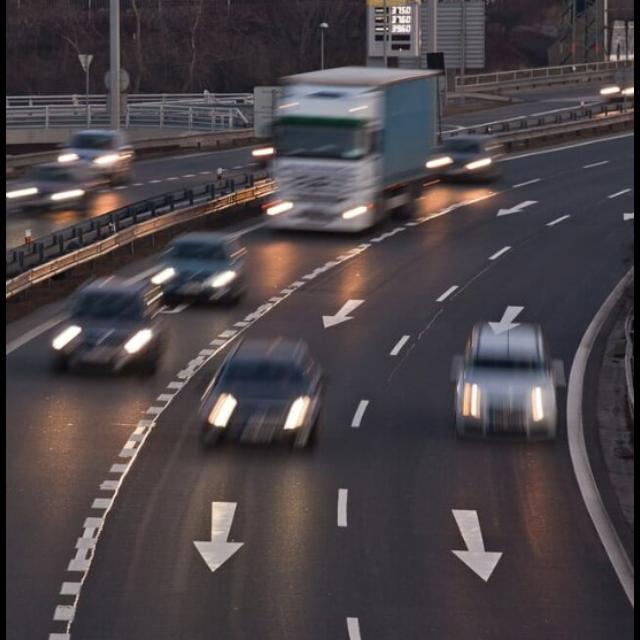
\includegraphics[width=\linewidth]{tex/img/train-1.jpg}
    \caption{Image-1: from Training dataset}
    \label{fig:tain-1}
  \end{minipage}%
  \begin{minipage}{0.5\textwidth}
    \centering
    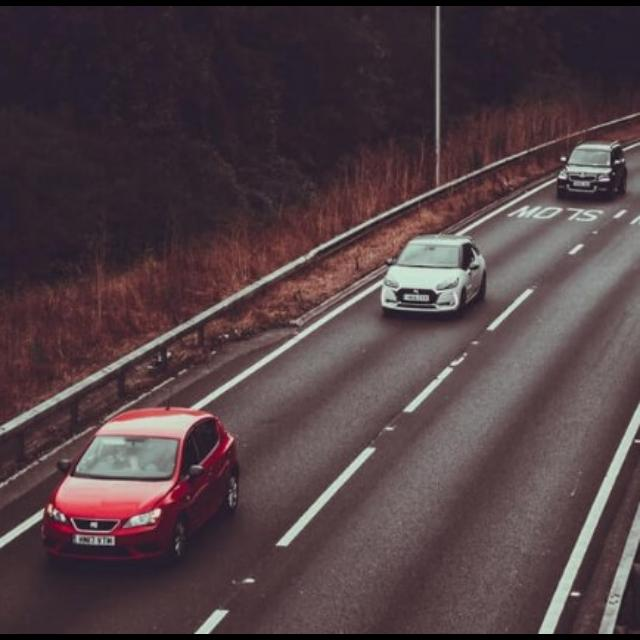
\includegraphics[width=\linewidth]{tex/img/train-2.jpg}
    \caption{Image-1: from Training dataset}
    \label{fig:train-2}
  \end{minipage}
  \begin{minipage}{0.5\textwidth}
    \centering
    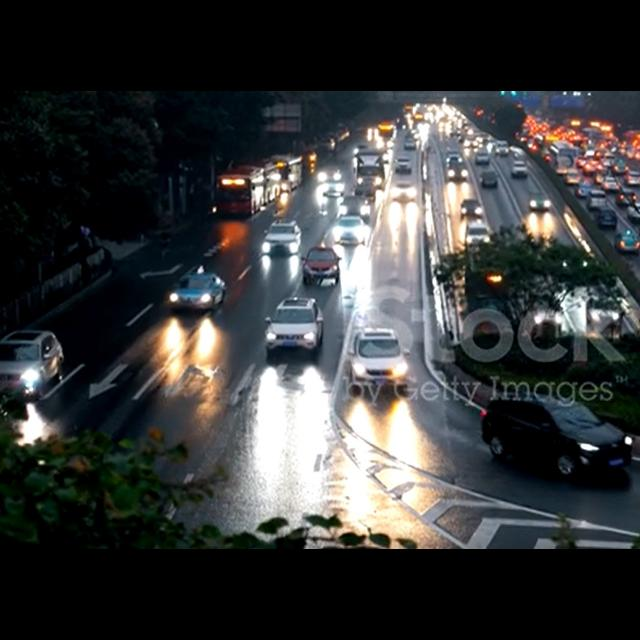
\includegraphics[width=\linewidth]{tex/img/valid-1.jpg}
    \caption{Image-1: from validation dataset}
    \label{fig:valid-1}
  \end{minipage}
    \begin{minipage}{0.5\textwidth}
    \centering
    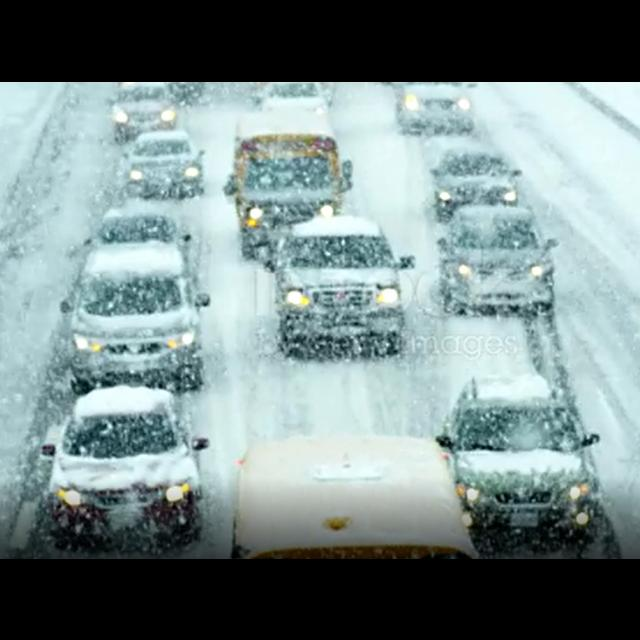
\includegraphics[width=\linewidth]{tex/img/valid-2.jpg}
    \caption{Image-1: from validation dataset}
    \label{fig:valid-2}
  \end{minipage}
  \caption{Sample image from dataset I am going to fine-tune} 
\vspace{3mm}
  The image used to test the model is completely different from the dataset. Source: \href{https://www.istockphoto.com/pl/zdj%C4%99cie/wiele-samochod%C3%B3w-na-drodze-gm490081958-75026541}{iStock}
\end{figure}  
After fine-tuning and extensive training, we will test our models on a set of images obtained from iStock image stocks. The test dataset comprises a variety of images with different object sizes, orientations, and backgrounds. Some samples of our test dataset are provided in the figure below.

\begin{figure}[H]
  \begin{minipage}{0.48\textwidth}
    \centering
    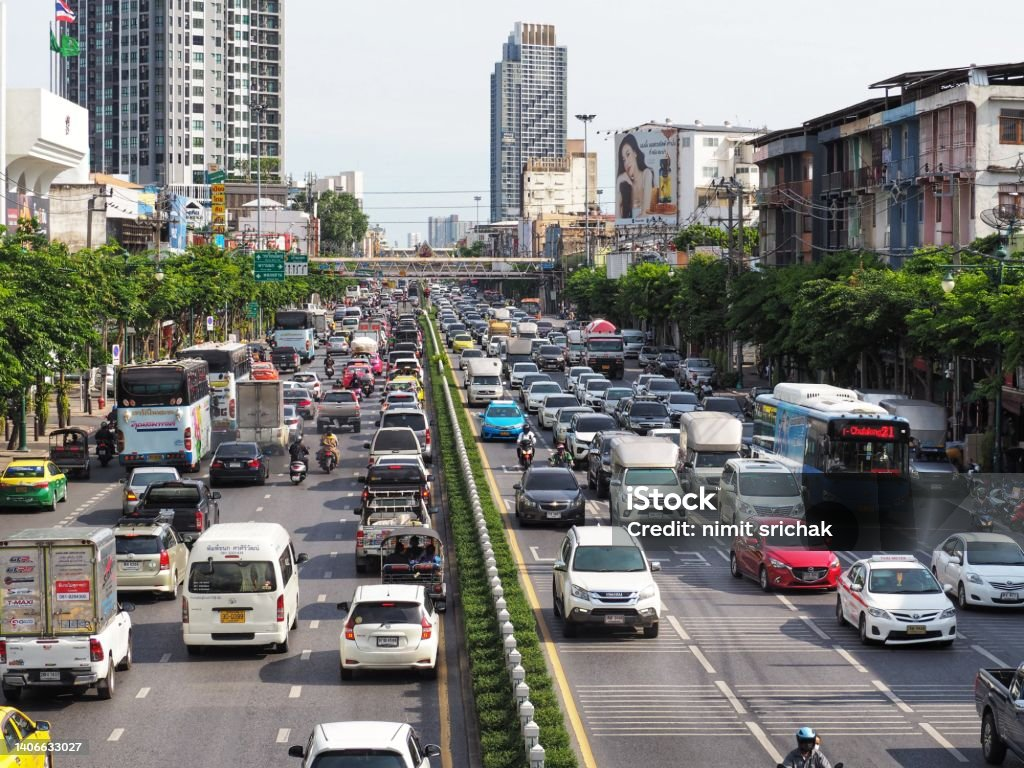
\includegraphics[width=\linewidth]{tex/img/car-1.jpg}
    \caption{Car-1}
    \label{fig:YOLO-NASSM_vs_other_models}
  \end{minipage}%
  \begin{minipage}{0.5\textwidth}
    \centering
    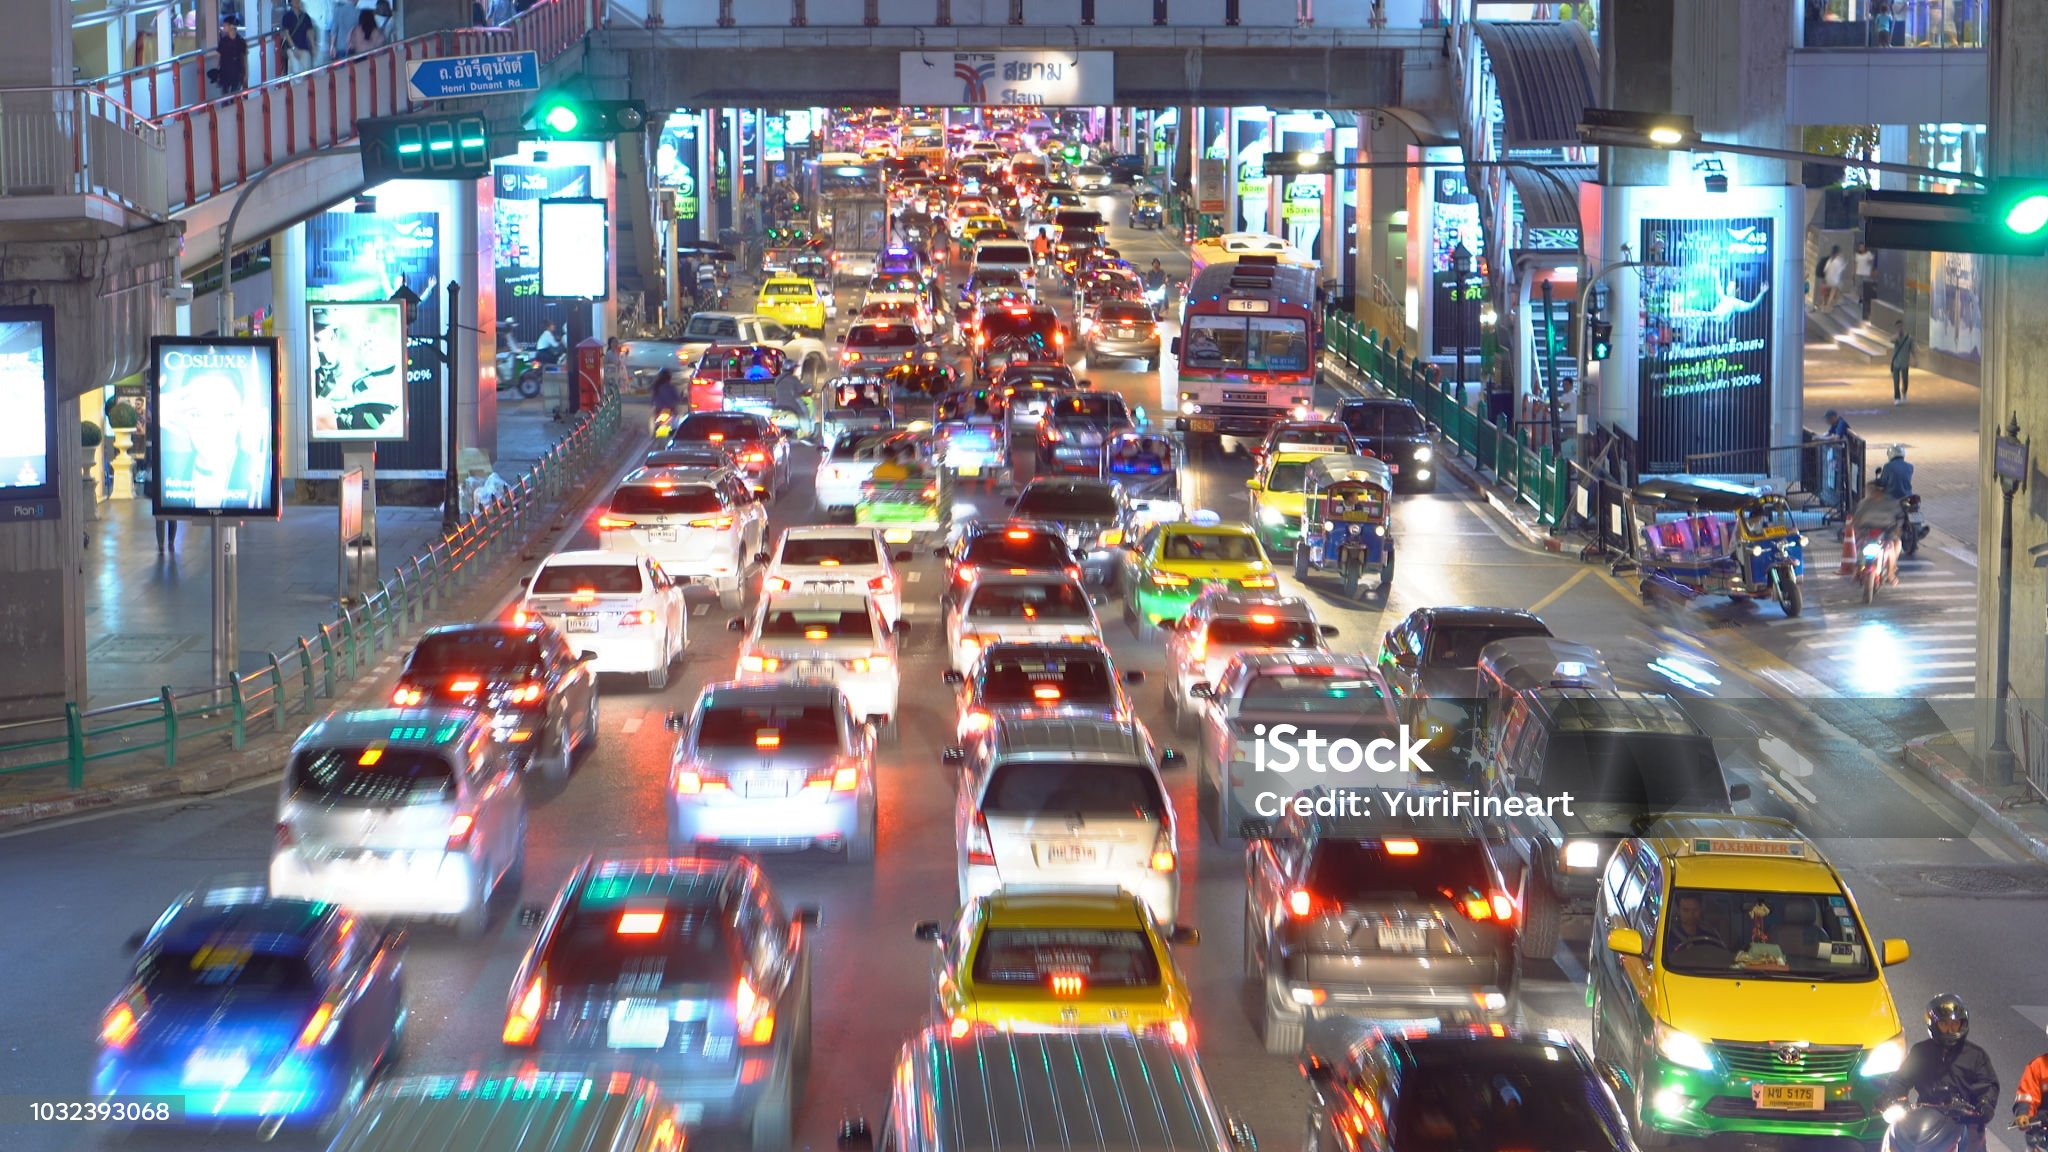
\includegraphics[width=\linewidth]{tex/img/car-4.jpg}
    \caption{Car-2}
    \label{fig:YOLO-NAS_vs_other_models}
  \end{minipage}
  \begin{minipage}{0.5\textwidth}
    \centering
    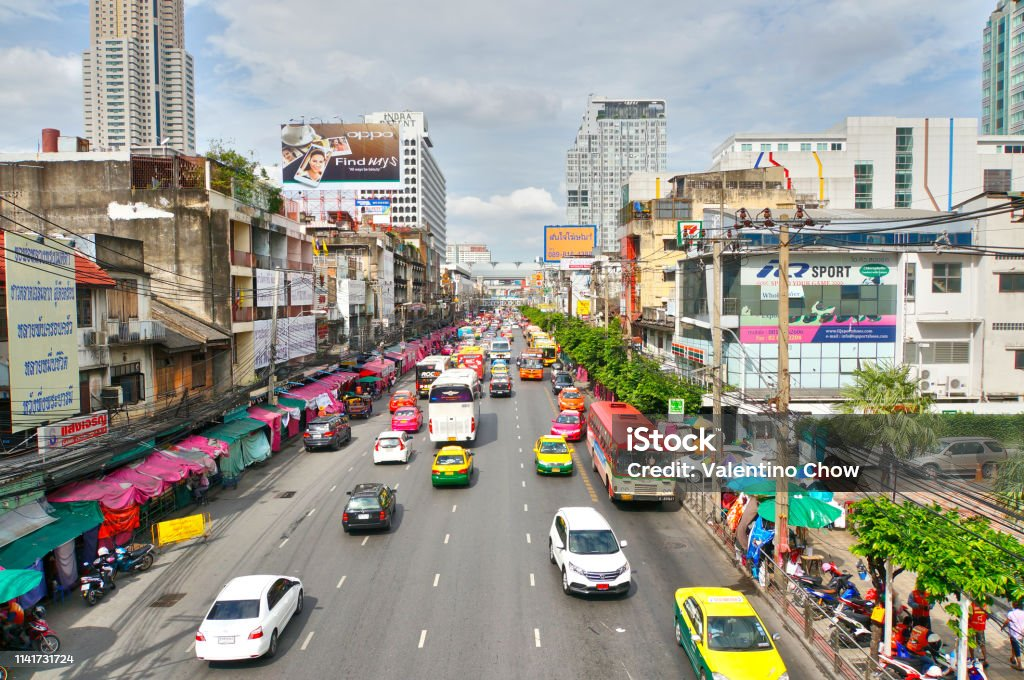
\includegraphics[width=\linewidth]{tex/img/car-8.jpg}
    \caption{Car-3}
    \label{}
  \end{minipage}
    \begin{minipage}{0.5\textwidth}
    \centering
    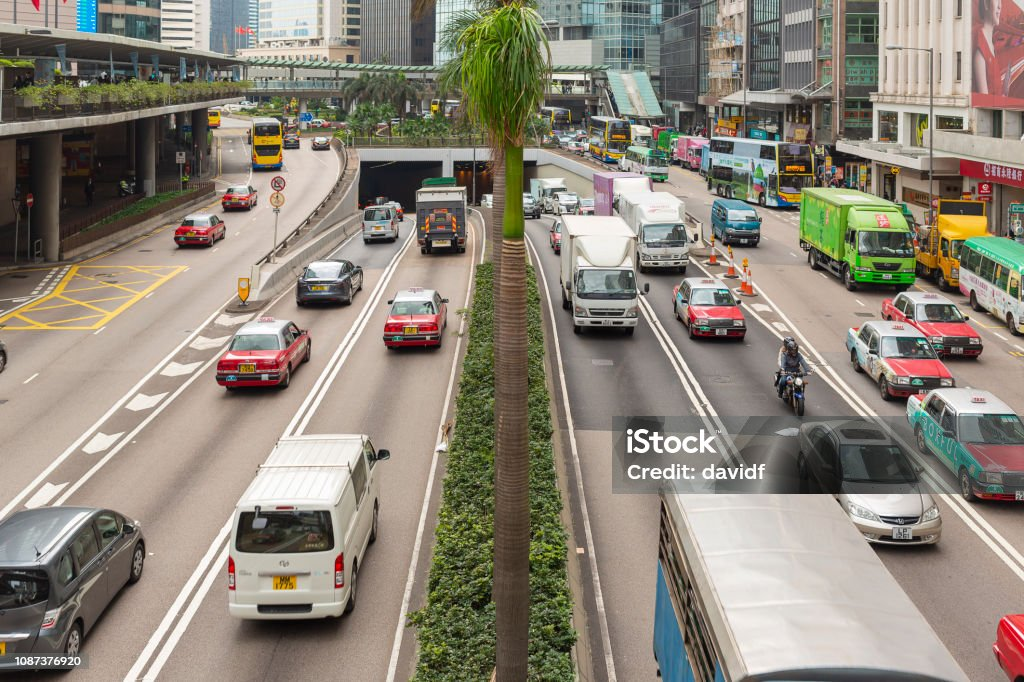
\includegraphics[width=\linewidth]{tex/img/car-11.jpg}
    \caption{Car-4}
    \label{}
  \end{minipage}
  \caption{Sample image for testing the model after and before the training. This image is taken from Istock by Getty Images for testing the model only.} 
\vspace{3mm}
  The image used to test the model is completely different from the dataset. Source: \href{https://www.istockphoto.com/pl/zdj%C4%99cie/wiele-samochod%C3%B3w-na-drodze-gm490081958-75026541}{iStock}
\end{figure}  
To train and test my models, I will utilize Google Colab, which provides powerful computers specifically designed for deep learning purposes. The machine I used for our experiments had an NVIDIA Tesla T4 GPU with high RAM, enabling us to train and test our models efficiently. 

Our experiments involved training the models on the training dataset and evaluating their performance on the validation and test datasets. I will analyze the models' performance based on various metrics, including mean average precision (mAP), accuracy, and time taken for inference. I will also compare the performance of YOLO-NAS variants.

The results of our study will shed light on the performance of YOLO-NAS and its variants on object detection tasks and provide insights into their strengths and weaknesses. This study will contribute to the development of more efficient and accurate object detection models that can be applied in various domains, including self-driving cars, surveillance systems, and robotics.
\subsection{YOLO}
YOLO (You Only Look Once) is an object detection system for real-time object detection. Ross Girshick, Ali Farhadi, Santosh Divvala, and Joseph Redmon were the ones who first introduced it in 2016. YOLO is known for its high speed and accuracy. The system is designed to classify and detect multiple objects in an image using a single forward pass of the neural network.
Traditional object detection systems use a sliding window approach where they apply a classifier at each location and scale of the image. This process is computationally expensive and time-consuming. On the other hand, YOLO divides the input image into a grid of cells, and each cell is responsible for detecting an object. This approach reduces the number of bounding boxes that need to be processed and allows for real-time detection; this makes it suitable for a wide range of applications such as self-driving cars, surveillance systems, and robotics. Additionally, YOLO can detect objects at different scales and aspect ratios, making it robust to variations in object size and orientation. \cite{terven2023comprehensive} \cite{redmon2016you} 

\subsection{The Evolution of YOLO}
\begin{figure}[H]
    \centering
    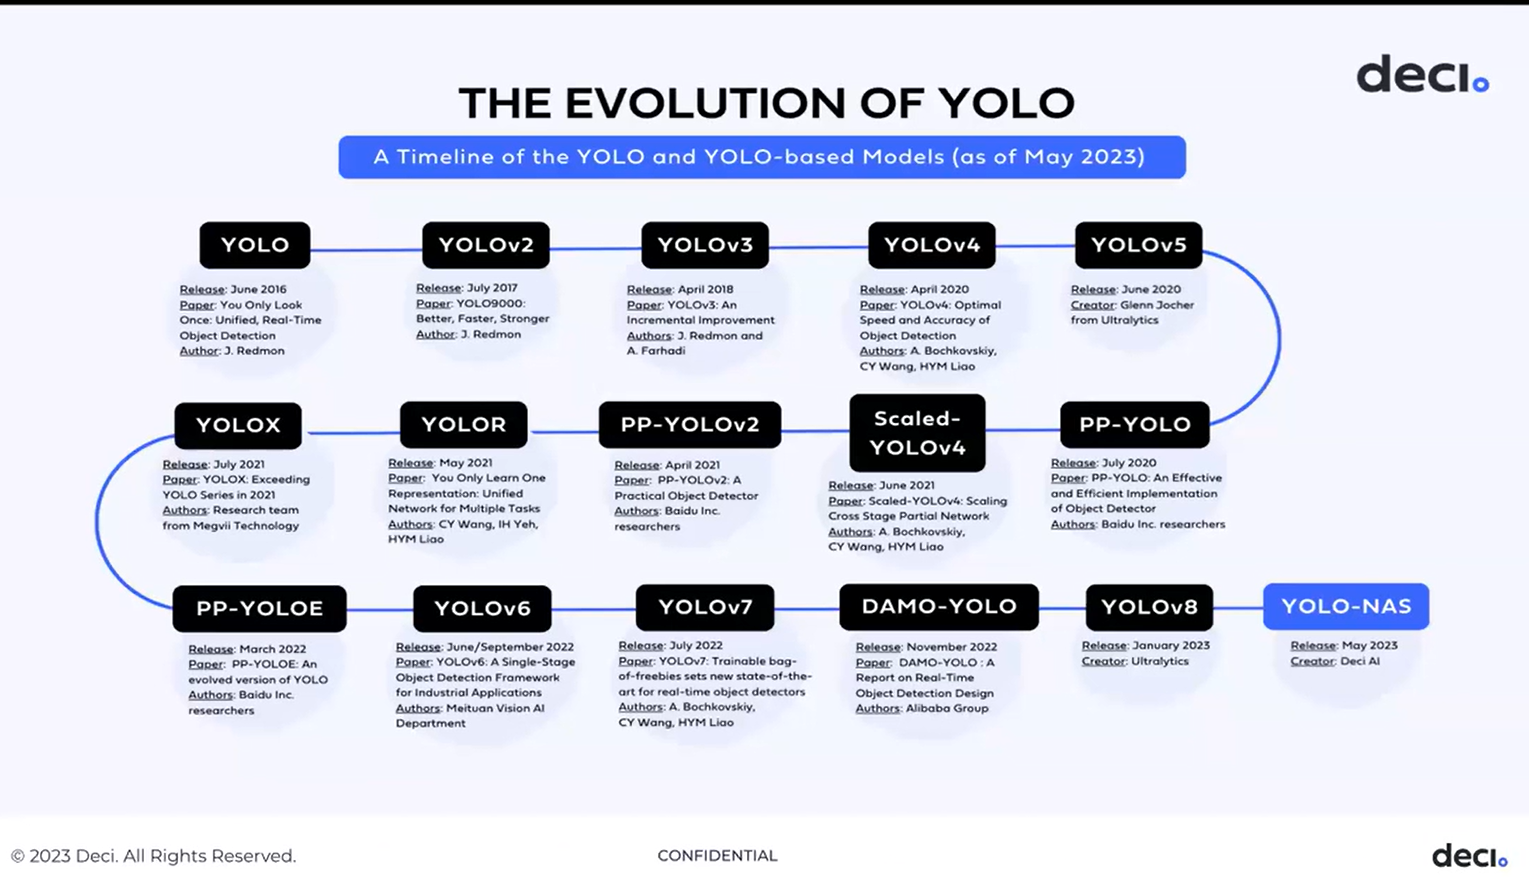
\includegraphics[width=\textwidth]{evolution_of_YOLO.PNG}
    \caption{The evolution  of yolo [Source: \href{https://deci.ai/resources/webinar-open-source-llms-vs-apis/}{\textcolor{black}{Deci. ai webinar}}]}
    \label{fig:YOLO-Evolution}
\end{figure}
\begin{enumerate}
    \item \textbf{YOLO: } YOLO was introduced in 2016 for real-time object detection.
    Achieved a groundbreaking mAP of 63.4\% on the PASCAL VOC2007 dataset.
    YOLO's efficiency in one network pass. Localization error limitations due to object count, aspect ratios, and down-sampling. \cite{redmon2016you}\\
    \item \textbf{YOLOv2 Improvements: } YOLOv2 was introduced in 2017 with 9000+ categories.
    Improved with batch normalization, high-resolution classifiers, and anchor boxes.
    Joint training for classification and detection.\cite{sang2018improved}\\
    \item \textbf{YOLOv3 Advancements: } YOLOv3 (2018) achieved 60.6\% mAP on MS COCO, 2x faster than previous versions.
    Introduced logistic regression for objectness scores and anchor box priors. \cite{redmon2018yolov3}\\
    \item \textbf{YOLOv4 Global Impact: } YOLOv4 (2020) maintained YOLO's philosophy with bag-of-freebies and bag-of-specials. Enhanced accuracy with image adjustments like mosaic augmentation and DropBlock. \cite{gai2023detection}
    \item \textbf{YOLOv5 Speed and Efficiency: } YOLOv5 (2020) by Ultralytics in PyTorch achieved 50.7\% AP with user-friendly features. \cite{wu2021real}\\
    \item \textbf{YOLOX Anchor-Free Innovation: } YOLOX (July 2021) exceeded previous YOLO versions, anchor-free with center sampling. Employed MixUP, Mosaic augmentations for improved accuracy. \cite{ge2021yolox}\\
    \item \textbf{YOLOR Multi-Task Learning: } YOLOR (May 2021) focused on a unified network for multiple tasks.
    Applied multi-task learning for classification, detection, and pose estimation.\\

    \item \textbf{PP-YOLOv2: }  Upgrades include ResNet101, PAN, Mish Activation, increased input size, and modifications to IoU-aware branch. \cite{huang2021pp}\\
    \item \textbf{Scaled-YOLOv4 Flexibility: } Scaled-YOLOv4 (CVPR 2021) introduced scaling-up and scaling-down techniques. YOLOv4-tiny for low-end GPUs, YOLOv4-large for cloud GPUs. \cite{wang2021scaled}\\ 
    \item \textbf{PP-YOLO: } A YOLOv3-based model by Baidu, leveraging PaddlePaddle, introducing ten tricks for accuracy without sacrificing speed.\cite{long2020pp}\\
    \item \textbf{PP-YOLOE: } Evolved from PP-YOLOv2 with anchor-free architecture, new backbone, TAL, ET-head, and VFL/DFL. \cite{xu2022pp}\\
    \item \textbf{YOLOv6 Industrial Framework: } 
    YOLOv6 (September 2022) for industrial applications with anchor-free detection.
    YOLOv6-L achieved 52.5\% AP and 70\% AP50 at 50 FPS. \cite{li2022yolov6}, \cite{terven2023comprehensive}
    \item \textbf{YOLOv7 Speed and Accuracy: } YOLOv7 (July 2022) surpassed others in speed and accuracy.
    E-ELAN, model scaling, and "bag-of-freebies" approach for efficiency. \cite{wang2023yolov7}, \cite{terven2023comprehensive}\\
    \item \textbf{DAMO-YOLO Real-Time Improvements: } DAMO-YOLO (November 2022) by Alibaba for real-time object detection. 
    Introduced MAE-NAS, Efficient-RepGFPN, ZeroHead, and knowledge distillation. \cite{xu2022damo}\\
    \item \textbf{YOLOv8 :}
    YOLOv8 (January 2023) by Ultralytics with anchor-free prediction and faster NMS. Mosaic augmentation during training for improved accuracy.
    YOLOv8 offers five scaled versions: YOLOv8n (nano), YOLOv8s (small), YOLOv8m (medium), YOLOv8l (large), and YOLOv8x (extra\-large). YOLOv8x outperformed YOLOv5 on the MS COCO dataset with an impressive 53.9\% AP at 640 pixels and fast speed.\cite{yolov8}, \cite{terven2023comprehensive}
\end{enumerate}

\subsection{YOLO-NAS}
YOLO-NAS is a cutting-edge object detection model created using Deci's Neural Architecture Search technology, AutoNAC™. It offers unmatched real-time object detection capabilities and production-ready performance, surpassing other models such as YOLOv5, YOLOv6, YOLOv7, and YOLOv8.

The YOLO-NAS model undergoes a multi-phase training process that involves pre-training on Objects365, COCO Pseudo-Labeled data, Knowledge Distillation (KD), and Distribution-Focal-Loss (DFL).

During the pre-training phase, the model is trained on Objects365, a comprehensive dataset that consists of 2 million images and 365 categories. Depending on the model variant, this process can take 25-40 epochs, as each epoch requires 50-80 minutes on 8 NVIDIA RTX GPUs. 

The COCO dataset offers an additional 123,000 images without labels. These images are utilized to create pseudo-labeled data. First, an accurate model is trained on COCO to label these images. Then, the labeled images are used to train our model alongside the 118,000 train images.

The YOLO-NAS architecture incorporates Knowledge Distillation (KD) and Distribution Focal Loss (DFL) techniques to improve its training process. Furthermore, the YOLO-NAS training procedure employs various datasets, including both labeled and unlabeled data, as well as supervised and unsupervised training methods.\cite{YOLO-NAS}, \cite{terven2023comprehensive}
\begin{figure}[H]
    \centering
    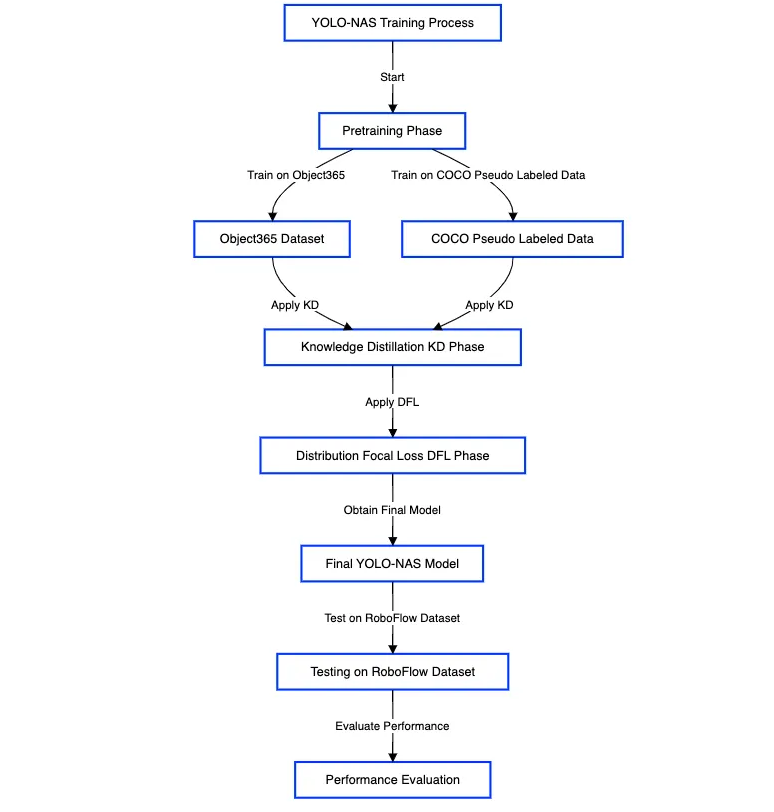
\includegraphics[width=0.8\textwidth]{YOLO-NAS-Training.PNG}
    \caption{An overview of the YOLO-NAS training process \cite{richmond_yolo-nas}}
    \label{fig:enter-label}
\end{figure}


\subsubsection{Architectural Features of YOLO-NAS} \vspace{0mm}It is considered one of the most efficient object detection algorithms due to its unique architecture, which is designed to minimize the computational cost of the algorithm while maintaining high accuracy.
\begin{enumerate}
    \item \textbf{Quantization Aware Blocks and Selective Quantization: } 
        \begin{itemize}
            \item \textbf{Hybrid Quantization Method: } YOLO-NAS uses a mixed quantization method that includes both Quantization-Specific Parameters (QSP) and Quantization-Centric Initialization (QCI) blocks. These leverage re-parameterization and 8-bit quantization, inspired by Chu et al.'s methodology.
            \item  \textbf{Selective Quantization:} The model strategically quantizes specific parts rather than uniformly affecting all layers. This selective quantization balances accuracy and latency, addressing information loss, a common issue in standard quantization techniques.
                \item \textbf{Layer Selection Algorithm:} YOLO-NAS utilizes a sophisticated layer selection algorithm to decide which layers to quantize. It evaluates the impact of each layer on accuracy and latency, carefully considering the implications of toggling between 8-bit and 16-bit quantization.
                \item \textbf{Performance in Limited Resources:} Uniquely designed for environments with limited resources, YOLO-NAS ensures superior performance. Its optimized approach to quantization preserves accuracy while being efficient, striking a crucial balance for advanced object detection tasks.
        \end{itemize}
    \item \textbf{Detection Head: } A standout feature of YOLO-NAS is its detection head design, which predicts a distribution probability for size regression. This approach is particularly useful in scenarios where the object sizes vary significantly. YOLO-NAS is an object detection model that predicts a range of possible sizes instead of a single fixed size. This unique approach improves its accuracy in detecting objects of varying scales. In addition, YOLO-NAS uses a probabilistic approach to size regression which makes it suitable for knowledge distillation. This means that it facilitates a more nuanced transfer of knowledge from a complex, high-capacity teacher model to a simpler, more efficient student model. All these features make YOLO-NAS a practical choice for diverse applications.
    \item \textbf{Neck: } The YOLO-NAS network has a highly advanced pyramid-attention neck that combines both top-down and bottom-up information flows. 
    \begin{figure}[H]
        \centering
        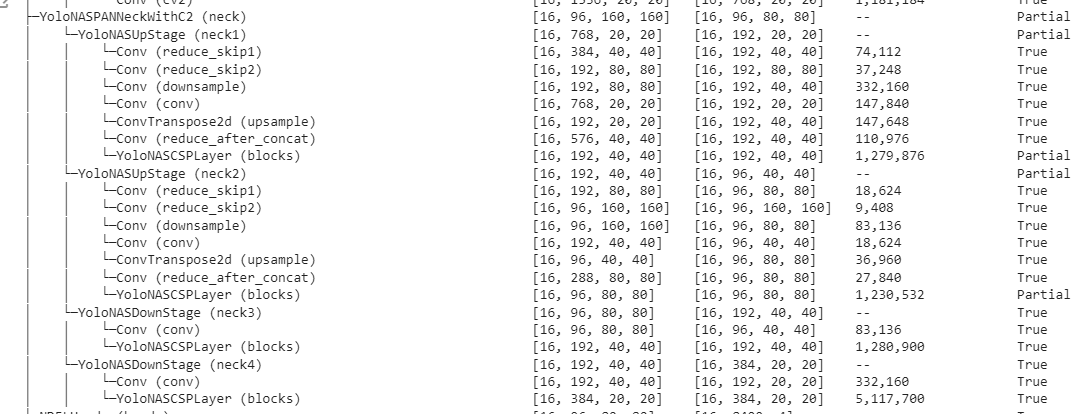
\includegraphics[width=\textwidth]{yolo-nas_neck.PNG}
        \caption{Neck Design}
        \label{fig:Neck}
    \end{figure}
    This design element assists the network in effectively capturing and utilizing multi-scale information. In this pyramid-attention structure, the top-down pathway captures high-level semantic information, while the bottom-up pathway focuses on smaller details. The attention mechanism in this pyramid structure ensures that the network focuses on the most relevant features at different scales, which improves its ability to detect objects with varying sizes and complexities. 
    \item \textbf{Backbone: } 
The backbone of YOLO-NAS is a significant component of its architecture, which is the result of an advanced Network Architecture Search (NAS) process. The process utilizes Deci's proprietary NAS technology, AutoNAC, to tailor the network structure for object detection tasks with unparalleled precision. This innovative approach ensures that the network structure meets the specific demands of the tasks at hand.
\begin{itemize}
    \item \textbf{quantization-aware RepVGG: } During the NAS process, they have incorporated quantization-aware RepVGG blocks into the model architecture, ensuring that our model architecture would be compatible with Post-Training Quantization (PTQ).\\
    \item \textbf{Spatial Pyramid Pooling (SPP): } YOLO-NAS backbone has Spatial Pyramid Pooling (SPP)  at the end to capture global context; it is a pooling layer that removes the fixed-size constraint of the network, i.e., a CNN does not necessitate a fixed or predetermined picture size input. Placing SPP at the end of the YOLO-NAS backbone allows the model to capture global context information, which is crucial for understanding the overall context of the scene. This can be beneficial for detecting objects that may span a larger region in the image.\cite{YOLO-NAS}
\end{itemize}

\href{https://deci.ai/blog/yolo-nas-object-detection-foundation-model/}{Source}

\begin{figure}[H]
    \centering
    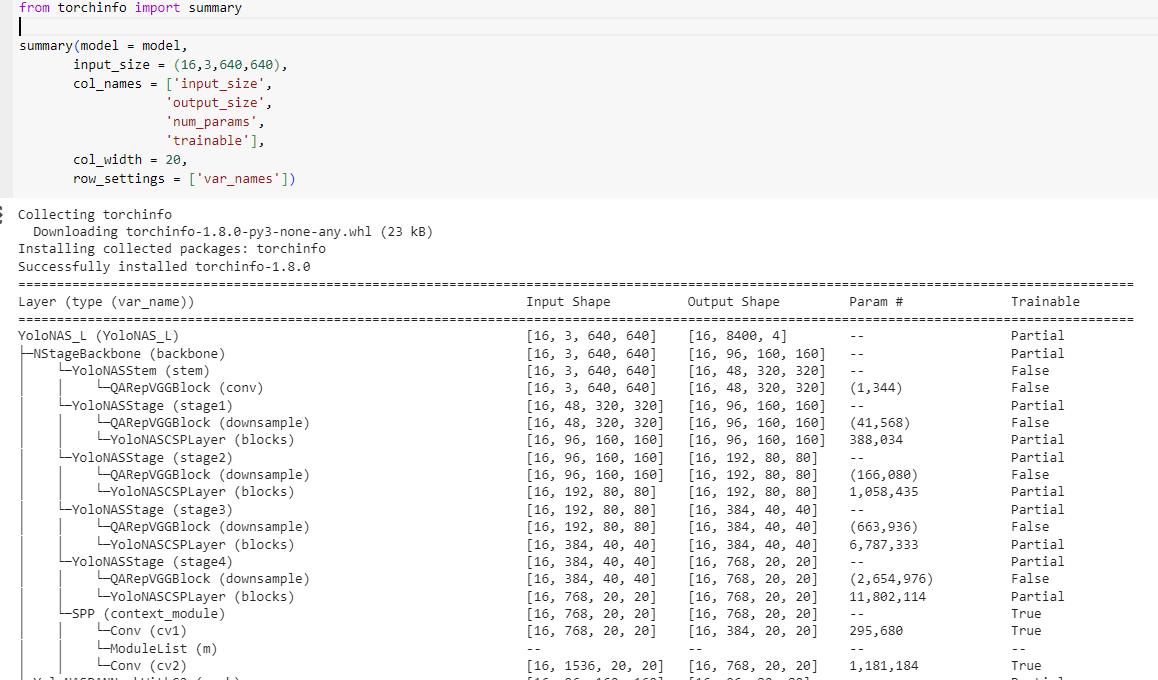
\includegraphics[width=\textwidth]{Yolo-BackBone.PNG}
    \caption{Backbone Structure}
    \label{fig:BackBone}
\end{figure}

AutoNAC plays a crucial role in the NAS process by determining the optimal sizes and structures of different stages in the YOLO-NAS backbone. This involves configuring the block type, number of blocks, and channels in each stage meticulously. Consequently, AutoNAC guarantees that every part of the backbone is meticulously optimized for its specific function. The NAS-generated backbone is not just a result of automated design but also of intelligent decision-making that considers various factors such as computational efficiency, accuracy, and speed. This ensures that the backbone contributes effectively to the overall robustness and adaptability of YOLO-NAS. These advancements lead to a superior architecture with exceptional object detection capabilities and outstanding performance compared to its predecessors.
\end{enumerate} 

\subsubsection{Automated Neural Architecture Construction (AutoNAC) engine}
Deci created the optimization engine AutoNAC, which Deci-AI uses. This engine applies Neural Architecture Search (NAS) to enhance the architecture of a deep learning model. The main goal is to improve the performance of the model when it is executed on specific hardware while maintaining or even improving its accuracy. The AutoNAC engine is hardware aware, data-aware and considers all the components in the inference stack, including compilers and quantization. \\
AutoNAC is essentially a NAS engine takes three components as inputs. \cite{yolo-nas-webinar}
\begin{itemize}
    \item \textbf{Task: } Firstly, we need to decide which model to build, such as an object detection model.\\
    \item \textbf{Data characteristics: } Deci Group requires the NAS Engine to be data-aware or capable of understanding the characteristics of the data so that it can create a model that is well-suited for the task at hand. For instance, if the objective is to detect small objects, the model would likely be different from that required for detecting large objects, as the receptive fields would differ. \\
    \item \textbf{Inference environment and Hardware: } When it comes to computer vision on edge, the priority is to achieve real-time performance or improve some level of latency or throughput while being hardware-aware, compilation-aware, and quantization-aware. To achieve this, we need to consider factors such as model size, latency, and throughput. Decis Group's goal is to optimize these factors as part of the Neural Architecture Search (NAS) process. Manually finding the optimal architecture for object detection models can be a laborious and inefficient process. To address this issue, Deci utilized AutoNAC, a tool that uses neural design space incorporating state-of-the-art (SOTA) architectural design principles and Deci's novel neural elements, to discover novel object detection models. These models were optimized to minimize inference latency computed over NVIDIA's T4 cloud GPU, which is a widely used computing device. We achieve this by feeding all three inputs into the AutoNAC engine, which generates a new architecture.
\end{itemize}
 
\begin{figure}[H]
    \centering
    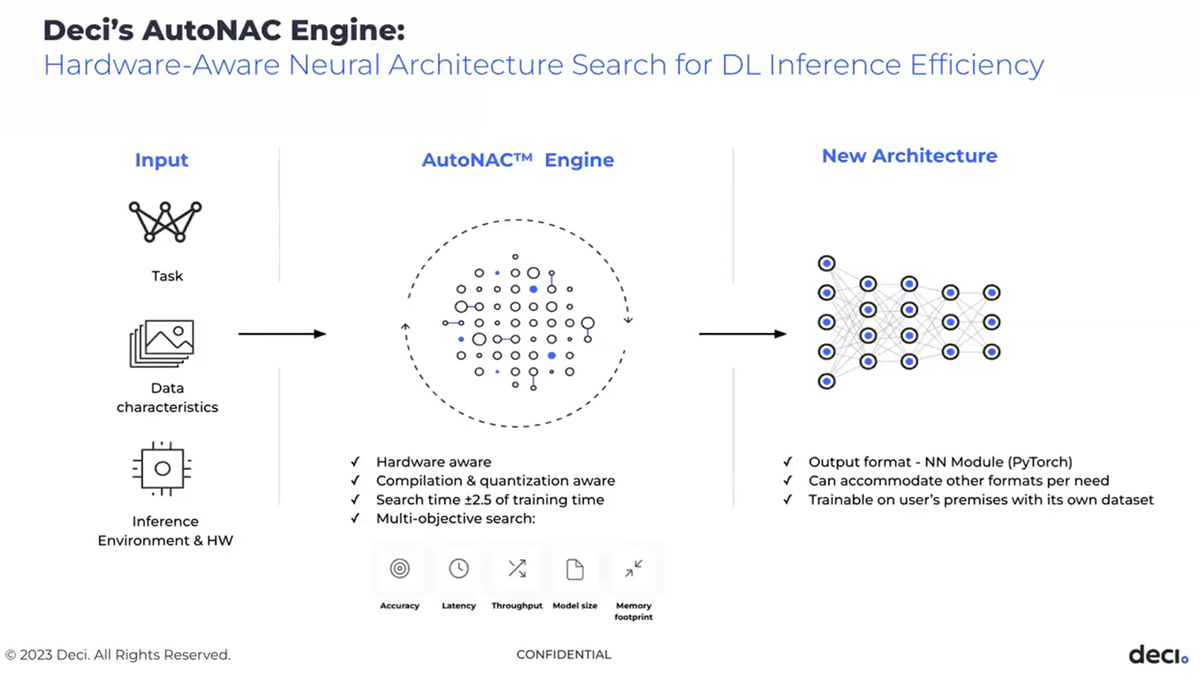
\includegraphics[width=\textwidth]{autoNAC_Engine.PNG}
    \caption{Deci's AutoNAC Engine; \\
    Hardware-Aware Neural Architecture Search for DL Inference Efficiency \cite{YOLo_NAS_Whitepaper_2022}\cite{yolo-nas-v8-sota}}
    \label{fig:AutoNAC Engine}
\end{figure}

\subsubsection{Under the hood View of Auto-NAC}
NAS algorithms can methodically search through the vast space of potential architectures, effectively locating novel and optimized configurations that human intuition might miss. By automating the process, these algorithms can quickly evaluate and compare an unimaginably large number of candidate architectures. They will eventually find a solution that strikes the best balance between accuracy, speed, and complexity. The NAS engine will be used when we already have data and want to build a model.
it takes all three inputs mentioned above, and the search space is automatically created under the hood, considering all the possibilities of neural architecture as an input. For example, optimal sizes, block types, number of blocks, and channel counts in every stage. \cite{yolo-nas-webinar} \cite{YOLo_NAS_Whitepaper_2022}
\begin{figure}[H]
    \centering
    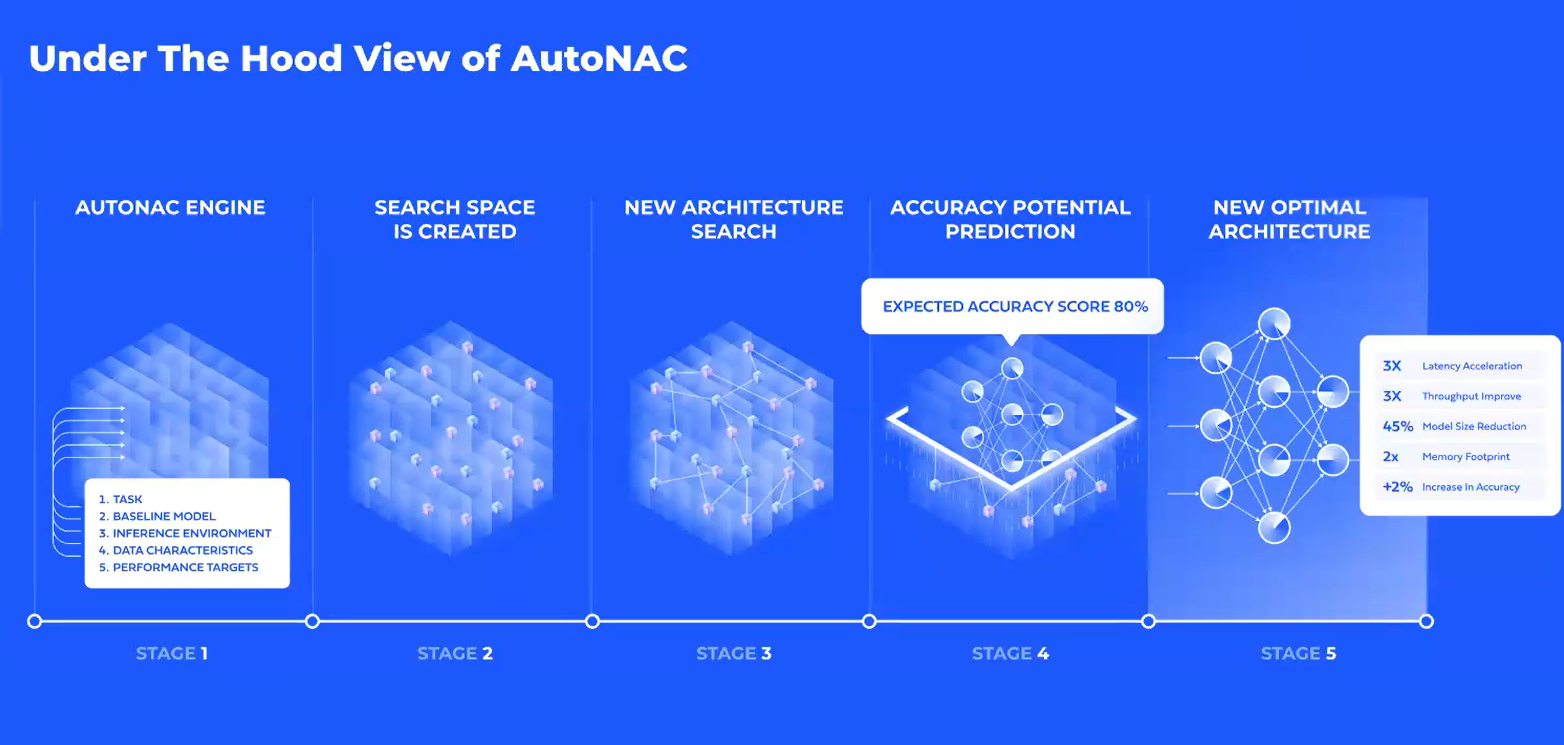
\includegraphics[width=\textwidth]{AUTONACENGINE_Underthe hood.PNG}
    \caption{AutoNAC Engine Search Space \cite{yolo-nas-webinar}}
    \label{fig:autonac_under_the_hood}
\end{figure}
Finally, AutoNAC Engine explores and maps the efficiency frontier, searching for an architecture that best balances latency vs. throughput. Deci Group samples three points of this frontier to create the YOLO-NASS, YOLO-NASM, and YOLO-NASL architectures.
\subsubsection{How to find the best architecture out of the search space}
while the search space has trillions of candidate architectures, the task of identifying the optimal architecture becomes increasingly challenging. Within the realm of Deci, the selection of the most suitable candidate from the numerous models within the extensive search space is guided by two distinct evaluation criteria. \cite{yolo-nas-webinar}
\begin{enumerate}
    \item \textbf{Bench Marking: } Understanding how the model will behave on the expected hardware or using the techniques of Latency Vs. throughput for the candidate architecture. \\
    \item \textbf{Accuracy Potential Predictions: } The fundamental selection methodology of best candidate out of the search space involves the provision of an AI model, designated to assess the accuracy or potential accuracy of neural network models. Leveraging principles from neural architecture search, YOLO-NAS systematically navigates the expansive design space of possible neural network configurations, employing optimization algorithms to identify architectures anticipated to yield high accuracy on the specified object detection task.
\end{enumerate}
 \begin{figure}[H]
     \centering
     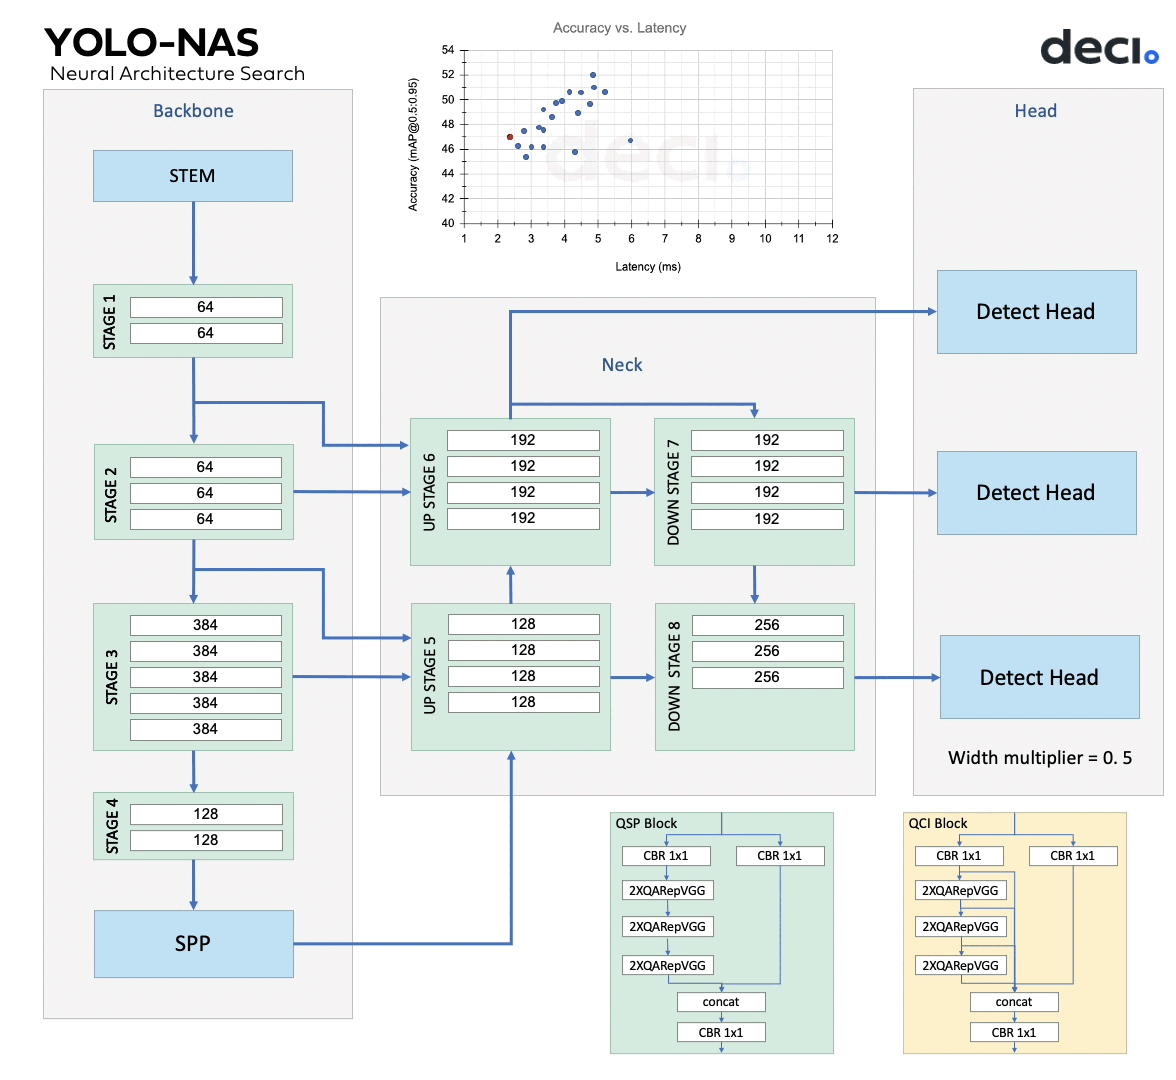
\includegraphics[width=\textwidth]{Yolo_nas.png}
     \caption{\textbf{YOLO-NAS Architecture \cite{YOLO-NAS}. The architecture is found automatically via a Neural Architecture Search(NAS) system called AutoNAC to balance latency vs. throughput. They generated three architectures called YOLO-NASS(small), YOLO-NASM(medium), and YOLO-NASL(large), varying the depth and the position of the QSP and QCI blocks \cite{YOLO-NAS}}}
     \label{fig:YOLO-NAS Architecture.}
\end{figure}


\subsubsection{Fine-tuning of the selected model On custom data set}
Fine-tuning refers to the process of making minor adjustments to achieve the desired output or performance. In deep learning, pre-existing trained neural networks can be used to program another deep learning algorithm from the same domain by using their weights. These weights are responsible for connecting each neuron in one layer to every neuron in the next layer of the neural network. Fine-tuning can be used to speed up the training process and overcome a small dataset as it already contains vital information from the pre-existing deep learning algorithm. The YOLO-NAS architecture and pre-trained weights are an excellent starting point for fine-tuning downstream tasks and define a new frontier in low-latency inference. When fine-tuning, using strong pre-trained weights often leads to higher model accuracy on new datasets. YOLO-NAS was trained on the RoboFlow100 dataset, which is a collection of 100 datasets from diverse domains, to demonstrate its ability to handle complex object detection tasks. The RF100 dataset is a benchmark for existing YOLO models, enabling us to compare YOLO-NAS's performance against them and showcase its advantages.\cite{YOLO-NAS}
\begin{figure}[H]
    \centering
    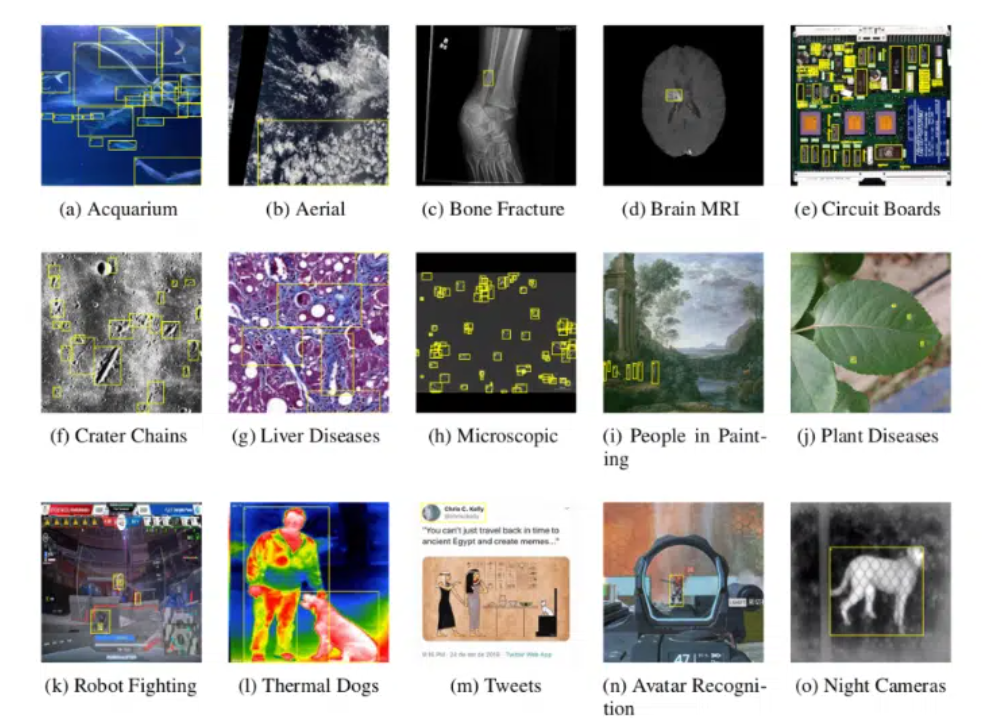
\includegraphics[width=0.8\textwidth]{YOLO-NAS_RF100_benchmark.PNG}
    \caption{Examples of annotated images in the RF100 benchmark \cite{YOLO-NAS}}
    \label{fig:YOLO-NAS_RF100_benchmark}
\end{figure}
The following hyperparameters ensure a robust and consistent training process, allowing for a fair comparison of the model’s performance across different datasets.\\
Deci followed the RF100 repository’s training protocol to ensure a fair comparison.\\
The model was trained for 100 epochs on a single T4 GPU with 16GB of VRAM, using consistent settings across all datasets.\cite{YOLO-NAS}, \cite{yolo-nas-vs-yolov8}
\begin{itemize}
    \item Learning rate: a learning rate of 5e-4 is used, while for the Medium version, the learning rate is set to 4e-4.
    \item Weight decay: 1e-4 (excluding bias and BatchNorm layers)
    \item Exponential moving average (EMA) with a decay factor of 0.99
    \item Batch size: 16
    \item Image resolution: 640×640
\end{itemize}


\begin{figure}[H]
  \begin{minipage}{0.48\textwidth}
    \centering
    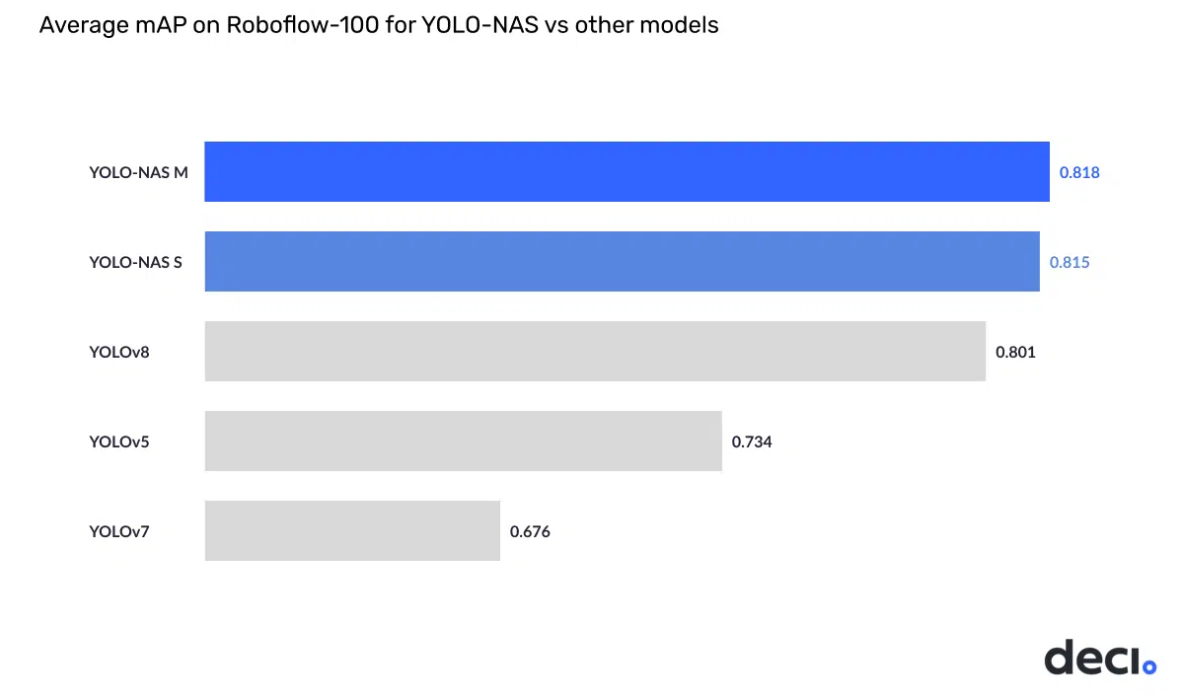
\includegraphics[width=\linewidth]{YOLO-NASSM_vs_other_models.PNG}
    \caption{Average mAP on Roboflow-100 \\for YOLO-NAS vs other models.}
    \label{fig:YOLO-NASSM_vs_other_models}
  \end{minipage}%
  \begin{minipage}{0.5\textwidth}
    \centering
    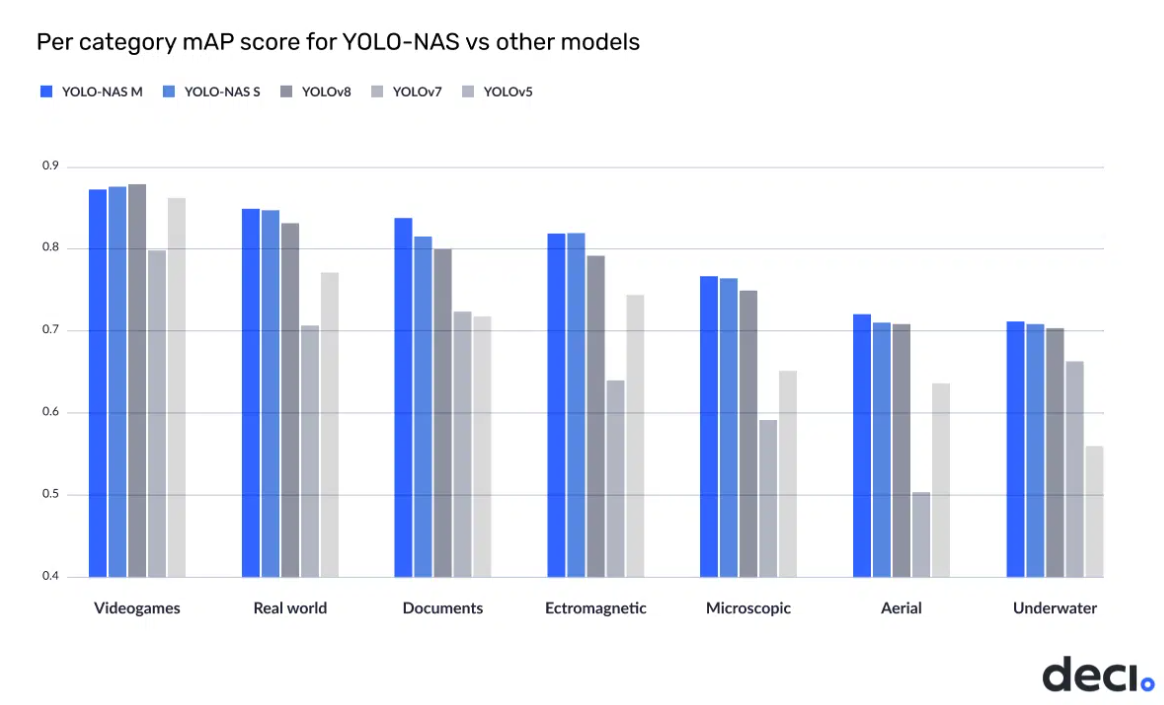
\includegraphics[width=\linewidth]{YOLO-NAS_vs_other_models.PNG}
    \caption{Per category mAP score for YOLO-NAS vs other models.
    Note: For Yolo vV5/v7/v8}
    \label{fig:YOLO-NAS_vs_other_models}
  \end{minipage}
  \caption{Average mAP and Per category mAP score for YOLO-NAS vs other models. \cite{YOLO-NAS}}
\end{figure}
Figure \ref{fig:YOLO-NASSM_vs_other_models} are the results obtained by focusing on the “Small” and “Medium” YOLO-NAS variants, and figure: \ref{fig:YOLO-NAS_vs_other_models} is a per-category breakdown of YOLO-NAS’s performance on the RF-100 dataset, compared to the performance of v5/v7/v8 models. \cite{YOLO-NAS}, \cite{yolo-nas-v8-sota}
\subsubsection{Object Detection Evaluation Metrics}
Object detection metrics are measurements that are used to assess the effectiveness of object detection algorithms. These metrics are essential in determining the accuracy and efficiency of object detection models, as they provide insights into the model's ability to identify and locate objects within images. Furthermore, they help in identifying false positives and false negatives. This information is critical in evaluating and improving the model's performance. There are many evaluation metrics that are applicable across different object detection algorithms, including the YOLO-NAS model. \cite{metrics}

\begin{itemize}
    \item \textbf{Intersection over Union (IoU):} Intersection over Union (IoU) is a fundamental measure that quantifies the overlap between a predicted bounding box and a ground truth bounding box. It plays a crucial role in evaluating the accuracy of object localization.
    \item \textbf{Average Precision (AP):} AP calculates the area under the precision-recall curve, producing a single value that encompasses precision and recall performance.
    \item \textbf{Mean Average Precision (mAP):} mAP calculates the average AP values across multiple object classes, making it useful in multi-class object detection scenarios for comprehensive model performance evaluation.
    \item \textbf{Precision and Recall:} Precision and Recall are two important metrics used to evaluate the performance of classification models. Precision measures the percentage of true positives among all positive predictions, indicating the model's ability to avoid false positives. Recall, on the other hand, calculates the percentage of true positives among all actual positives, indicating the model's ability to detect all instances of a class. These metrics are often used together to provide a more complete picture of a model's performance.
    \item F1 Score: The F1 Score is a measure of a model's performance that takes into account both precision and recall. It provides a balanced assessment while considering false positives and negatives.
\end{itemize}

\subsubsection{Benefits of YOLO-NAS over other models}
\textbf{Optimized Efficiency: }\\
YOLO-NAS is an advanced model that has been designed to achieve an optimal balance between accuracy and speed, making it more efficient than other human-designed models. This optimization is essential for real-time object detection applications as it enhances inference speeds and improves resource utilization. YOLO-NAS outperforms other models in terms of efficiency, making it the go-to choice for those who demand high-performance object detection capabilities." \\
\textbf{Adaptability to Diverse Tasks and Hardware: }\\
The architecture of YOLO-NAS allows it to adapt to various object detection tasks, including complex scenarios and hardware. Its versatility makes it a valuable tool across a wide range of applications.\\
\textbf{Training on Prominent Datasets: }\\
The architecture of YOLO-NAS allows it to adapt to various object detection tasks, including complex scenarios and hardware. Its versatility makes it a valuable tool across a wide range of applications.\\
\textbf{Detection and Localization Accuracy: }\\
The YOLO-NAS architecture is a specialized object detection model that addresses the challenges associated with detecting small or intricate objects. Its heightened detection capabilities and improved accuracy in pinpointing precise locations make it a superior choice for a diverse range of applications, particularly those where identifying small or elusive objects is crucial. In contrast, the YOLOv8 object detection model, while impressive, is limited in its ability to detect small objects accurately and localize them with precision. Despite its proficiency in various scenarios, YOLOv8 falls short when compared to the specialized capabilities of YOLO-NAS in handling the challenges posed by diminutive objects. \cite{yolo-nas-vs-yolov8}
\begin{figure}[H]
    \centering
    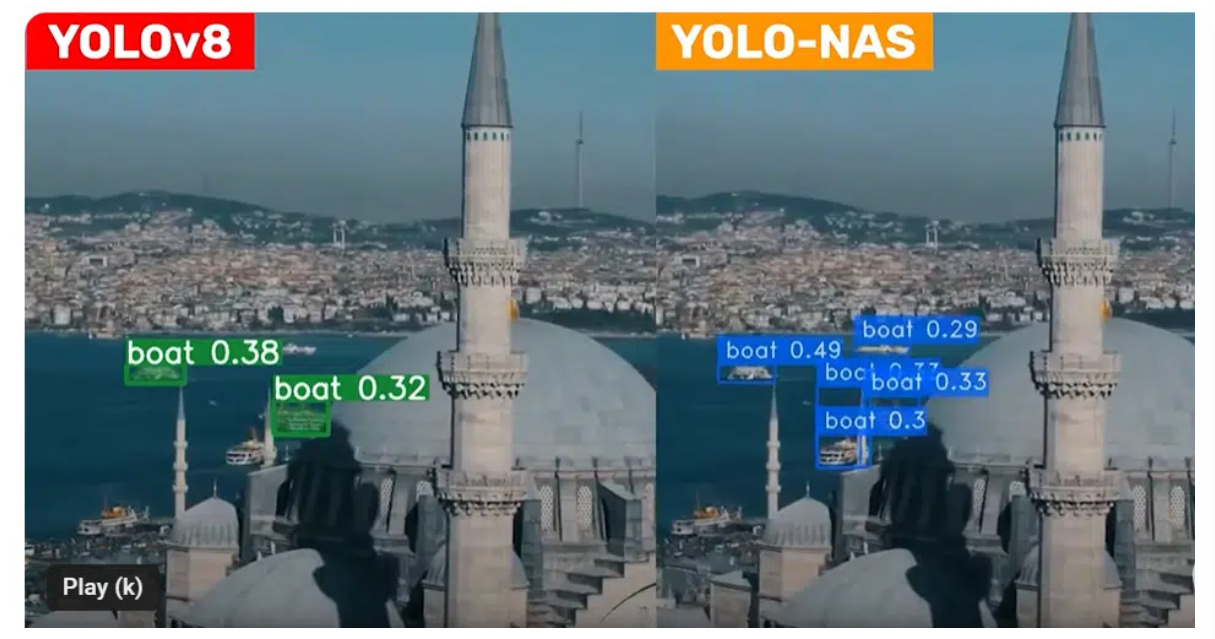
\includegraphics[width=0.7\textwidth]{YOLO-V8_vs_YOLO-NAS.PNG}
    \caption{Performance evaluation on YOLO-V8 vs. YOLO-NAS (\href{https://www.youtube.com/watch?v=uPgE8G4CGF4} Image Source: {\textcolor{black}{Youtube}})}
    \label{Yolo-V8_vs_YOLO-NAS}
\end{figure}


\subsubsection{Data set}
\label{datset}
The "Smart City Cars Detection Computer Vision Project" stands as a meticulously curated dataset within the Roboflow Universe, purposefully designed for object detection, with a specific emphasis on vehicular recognition. Encompassing various vehicle types, including buses, cars, motorbikes, and trucks this dataset plays a crucial role in advancing computer vision applications.
Regarding key attributes, the project adopts an object detection framework with distinct classes such as bus, car, motorbike, and truck. The dataset comprises 2753 after preprocessing applied from 1099 original images, with data allocation distributed as 90\texttt{\%} for training, 8\texttt{\%}for validation, and 2\texttt{\%} for testing.

During preprocessing, the image is resized to fit within a 640x640 frame, with black edges if necessary. Augmentations include rotating between -15° and +15°, shearing horizontally and vertically by ±15°, adjusting hue between -25° and +25°, saturating between -40\texttt{\%} and +40\texttt{\%}, applying blur up to 4 pixels, introducing noise up to 3\texttt{\%} of pixels, and utilizing mosaic augmentation. For bounding boxes, cropping ranges from 0\texttt{\%} minimum zoom to 20\texttt{\%} maximum zoom, and brightness is adjusted between -30\texttt{\%} and +30\texttt{\%}. The model generates three outputs per training example.

This dataset holds substantial utilitarian significance across various domains. It facilitates real-time traffic monitoring and analysis, contributing to Employing the Smart City Cars Detection model to process live video feeds of traffic, recognize various vehicle types and their numbers, and adjust traffic light timings dynamically. This optimization aims to reduce congestion and enhance the overall traffic flow within a smart city environment.   

Additionally, it Utilizes the Smart City Cars Detection model for monitoring parking areas, distinguishing between different vehicle classes occupying spaces (cars, trucks, buses, motorbikes), and offers drivers real-time updates on parking space availability through smart parking applications, Integrate findings from the Smart City Cars Detection model to analyze the distribution of diverse vehicle types in specific locations or across the entire city. This information aids city planners in devising focused infrastructure development plans, such as dedicated bus lanes, motorcycle parking, or optimized truck routes, Input the Smart City Cars Detection model data into machine learning algorithms for the autonomous generation of precise forecasts regarding future traffic patterns. This includes predicting peak hours and identifying locations prone to congestion, enabling proactive measures to be implemented. Mostly, Employ the Smart City Cars Detection model to observe bus utilization within a city, recognizing both bus occupancy and frequency. Utilize this information to enhance public transportation routes, determining whether additional buses or different types of public transport are required for more efficient service to the population.

The "Smart City Cars Detection Image Dataset" dataset epitomizes substantive potential across domains, ranging from traffic management and security to autonomous vehicles, fleet management, and traffic accident analysis.\cite{p4p-cars_dataset}

